%!TEX root = ../thesis.tex
\newchap{Event classification and signal extraction}\label{sec:signal}
\vspace{-1cm}
\minitoc
This chapter is focused on the signal-background discrimination. It will begin by demonstrating a basic one-dimensional feature ranking. Subsequently, JPANet will be adapted to tackle the signal-background discrimination challenge, and its score will be employed to execute a template fitting procedure on both the Muon and Electron channels, utilizing the Asimov dataset.
Once the statistical uncertainties associated with the $\PW \to cb$ rate are determined, we will also introduce and assess the systematic uncertainties and their impact on the signal rate extraction.
\begin{minipage}[H]{\linewidth}
\begin{minipage}{0.35\linewidth}
        \centering
        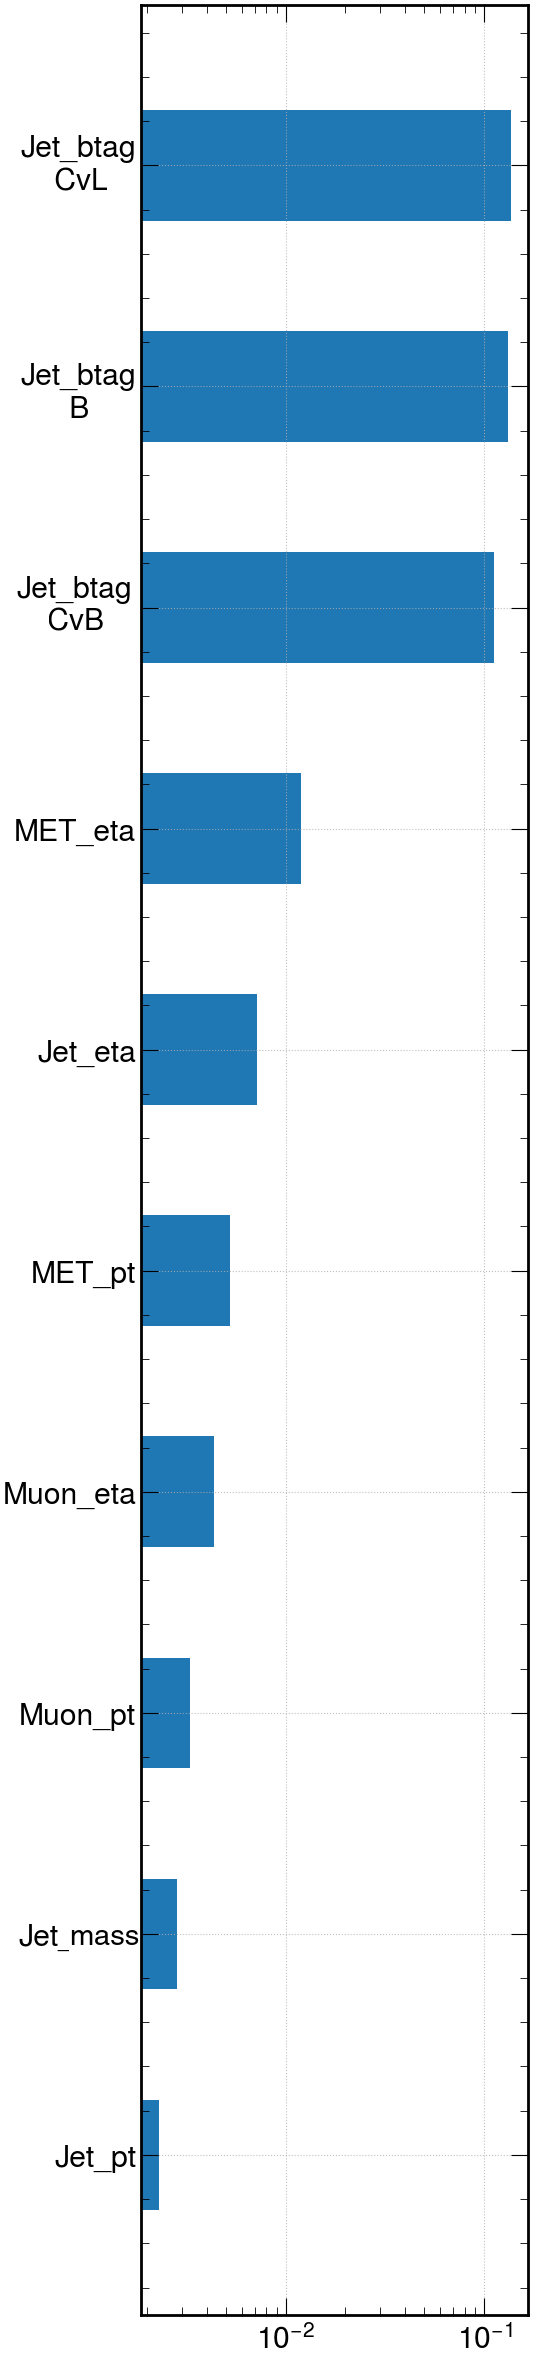
\includegraphics[height=0.7\textheight]{fig//chap08-kin_reco/ranking1D.png}
        
\end{minipage}
\hfill
\begin{minipage}{0.62\linewidth}
\vspace{-1cm}
\section{Unidimensional feature ranking}
To begin,  we can once again employ the metric $d$ to evaluate and rank the observables that discriminate the signal from the background.\\
\\
In this context, $d$ is computed between the signal and the $\ttbar$ semileptonic process, which is the primary source of background.\\
\\
All observables are treated as flattened, meaning that all objects within the events are combined in the same histograms, disregarding the event's inherent structure.\\
\\
The ranking process is carried out within the Muon channel following the initial preselection.\\
The results of this one-dimensional ranking are depicted in \Fig{fig:1Drank}.\\
\\
Notably, the observables with the highest ranking are those associated with b-tagging, exhibiting $d$ values of approximately 0.1.\\
Other observables produce results that are about an order of magnitude smaller, and the latests are due mostly to statistical fluctuations.

\end{minipage}
        \label{fig:1Drank}  
        \captionof{figure}{Unidimensional feature ranking using the metric $d$ between flattened signal observables and \ttbar semileptonic observables }
\end{minipage}
\section{Event classification}
\subsubsection*{SBANet} Since we have already demonstrated the ability of JPANet to reconstruct and interpret the signal events, we can exploit the same model to tackle the signal-background discrimination task.\\
To achieve this, we simply need to make some adjustments to JPANet, creating another network which will be denoted as "Signal-Background Attention Network" (SBANet).\\
The training and evaluation of this network will be conducted independently for the Muon and Electron channels.
\\
The differences between SBANet and JPANet are:\\
\\
\textbf{Jet Inputs}: In SBANet, all three \DeepJet scores are added to the Jet head (b-tag,CvB,CvL).
\\
\\
\textbf{Hyper-parameters}: After experimenting with various configurations, we found that the network required increased complexity. This entailed raising the number of units in each feed-forward layer to 128 and adjusting the dropout probability to 2\%.
\\
\\
\textbf{Self-attention pooling}: The JPANet's output initially produces a 7x4 matrix, as it assigns scores to pairs of jet-partons. However, we need to derive a single score for the entire event. To accomplish this, we condensed the physics objects embedding sequence into a single dimension using a self-attention pooling layer. This layer assigns weights to each element of the sequence (i.e., the physics objects) based on attention scores and computes a weighted average across the sequence. Subsequently, we introduced three additional feed-forward layers.
\\
\\
\textbf{Event self-attention}: We aimed to have the self-attention pooling calculate attention scores over all physics objects, not just the jets. Consequently, we transformed JPANet's cross-attention into a self-attention mechanism covering the concatenated sequence of jets and the leptonic W.
\\
\\
\textbf{Output layer} The output of SBANet is a 3-dimensional layer equipped with the softmax function. Three classes are defined: the signal, the $\ttbar$ semileptonic process, and the $\ttbar$ dileptonic process. This enables the network to better distinguish the signal from the two primary sources of background, even though, ultimately, we only consider the signal score.
\\  
\\
\textbf{Secondary leptons head} 
To enhance SBANet's ability to identify di-leptonic events, we introduced an additional head. In the muon(electron) channel, this head comprises a sequence of three elements: the second leading muon(electron), the leading and the second leading electron(muon).
The lepton features are limited to kinematic variables $(p_T,\eta,\phi)$, and the head is linked to a 2-layer feed-forward neural network.\\
The sequence of secondary leptons' embeddings is then combined with the complete event sequence before the self-attention pooling layer.
\\
\\
\textbf{Invariant mass heads and pair-wise attention biases} The two self-attention layers in the network were modified to include pair-wise physics object features, such as invariant masses.
Let's recall what is the scaled dot product:
\begin{equation}
    \text{Softmax}\left( \frac{QK}{\sqrt{d_k}} \right)V
\end{equation}
The product $QK$ is a $N\times N$ matrix where N is the length of the sequence.\\
Given that we can include the invariant masses of couples of physics objects by just adding a term in the softmax function
\begin{equation}
    \text{Softmax}\left( \frac{QK+\hat{M}}{\sqrt{d_k}} \right)V
\end{equation}
where $\hat{M}$ is a linear embedding of the matrix $M$ that contains all the invariant masses
\begin{equation}
\begin{aligned}
    M_{ij}&=\sqrt{(p_i+p_j)^\mu(p_i+p_j)_\mu} & \text{if } i\neq j\\
    M_{ij}&=m_i & \text{if } i=j\\
\end{aligned}
\end{equation}
The M matrix is symmetric and has $N(N+1)/2$ independent components.\\
The strategy to implement this in SBANet is adding another head containing for each event a vector of length 36 with the square invariant masses of the couple of jets and the leptonic W.
\begin{equation*}
    \text{Mass head inputs}=\Biggl[ \dboxed{m_W,m_{Wj_1},\:\dots\:,m_{Wj_7},\dboxed{m_{j_1},m_{j_1 j_2},\:\dots\:,m_{j_6},m_{j_6 j_7},m_{j_7}}}\: \Biggr]
\end{equation*}
This vector contains all the independent components of the M matrix.\\
Given the presence of significant outliers in the invariant masses, they are transformed with the function $\log(1+m)$ and then normalized with a batch norm layer.\\
Since the first self-attention layer works only on the jet sequence and the other on the jet + leptonic W sequence, we have to build two different mass embeddings.\\
\\
For jet-self attention, only the mass inputs that are not related to the leptonic W boson are considered. They are 28 elements that are fed to a 4-layer feed-forward neural network of size [28,128,128,28]. This network that has the same number of neurons in the first and the last layer is called Autoencoder.\\
The 28 output elements of the autoencoder are used to build the full $7\times 7$ M matrix that will be used as attention bias in the jet self-attention.\\
\\
The same thing is done with the event self-attention but considering all the mass head inputs and, in this case, the autoencoder size will be [36,128,128,36]\\


\begin{minipage}{\linewidth}
    \begin{minipage}{0.52\linewidth}
        \paragraph*{Training and evaluation}
        The network is trained and evaluated separately in the Muon and Electron channels. The dataset is divided into 85\% training and 15\% validation and is illustrated in \Tab{tab:SBANet_dataset}. \footnotemark\\
        To take into account the imbalance between the three classes, the cross-entropy loss function of SBANet is reweighted.
    \end{minipage}
    \hfill
    \begin{minipage}{0.45\linewidth}
        \centering
        \begin{tabular}{l|c|c}
            \toprule
             & \textbf{Training} & \textbf{Validation}\\
            \midrule
             signal& $9.1 \cdot 10^6$  & $1.6 \cdot 10^6$\\
             TTSL & $1.0 \cdot 10^8$ & $1.8 \cdot 10^7$\\
             TTDL & $2.0\cdot 10^7$ & $3.5 \cdot 10^6$\\
        \end{tabular}
        \captionof{table}{SBANet train and validation datasets before the Muon/Electron channel preselection.}
        \label{tab:SBANet_dataset} 
    \end{minipage}
\end{minipage}
\footnotetext{These events are not included in the effective MC luminosity shown in \Tab{tab:samples}. These are additional events used only to train and validate the network}\\
The loss functions of both the training and validation datasets are shown in \Fig{fig:SBANET_loss} and don't show any sign of overfitting.


\begin{figure}[H]
    \centering
    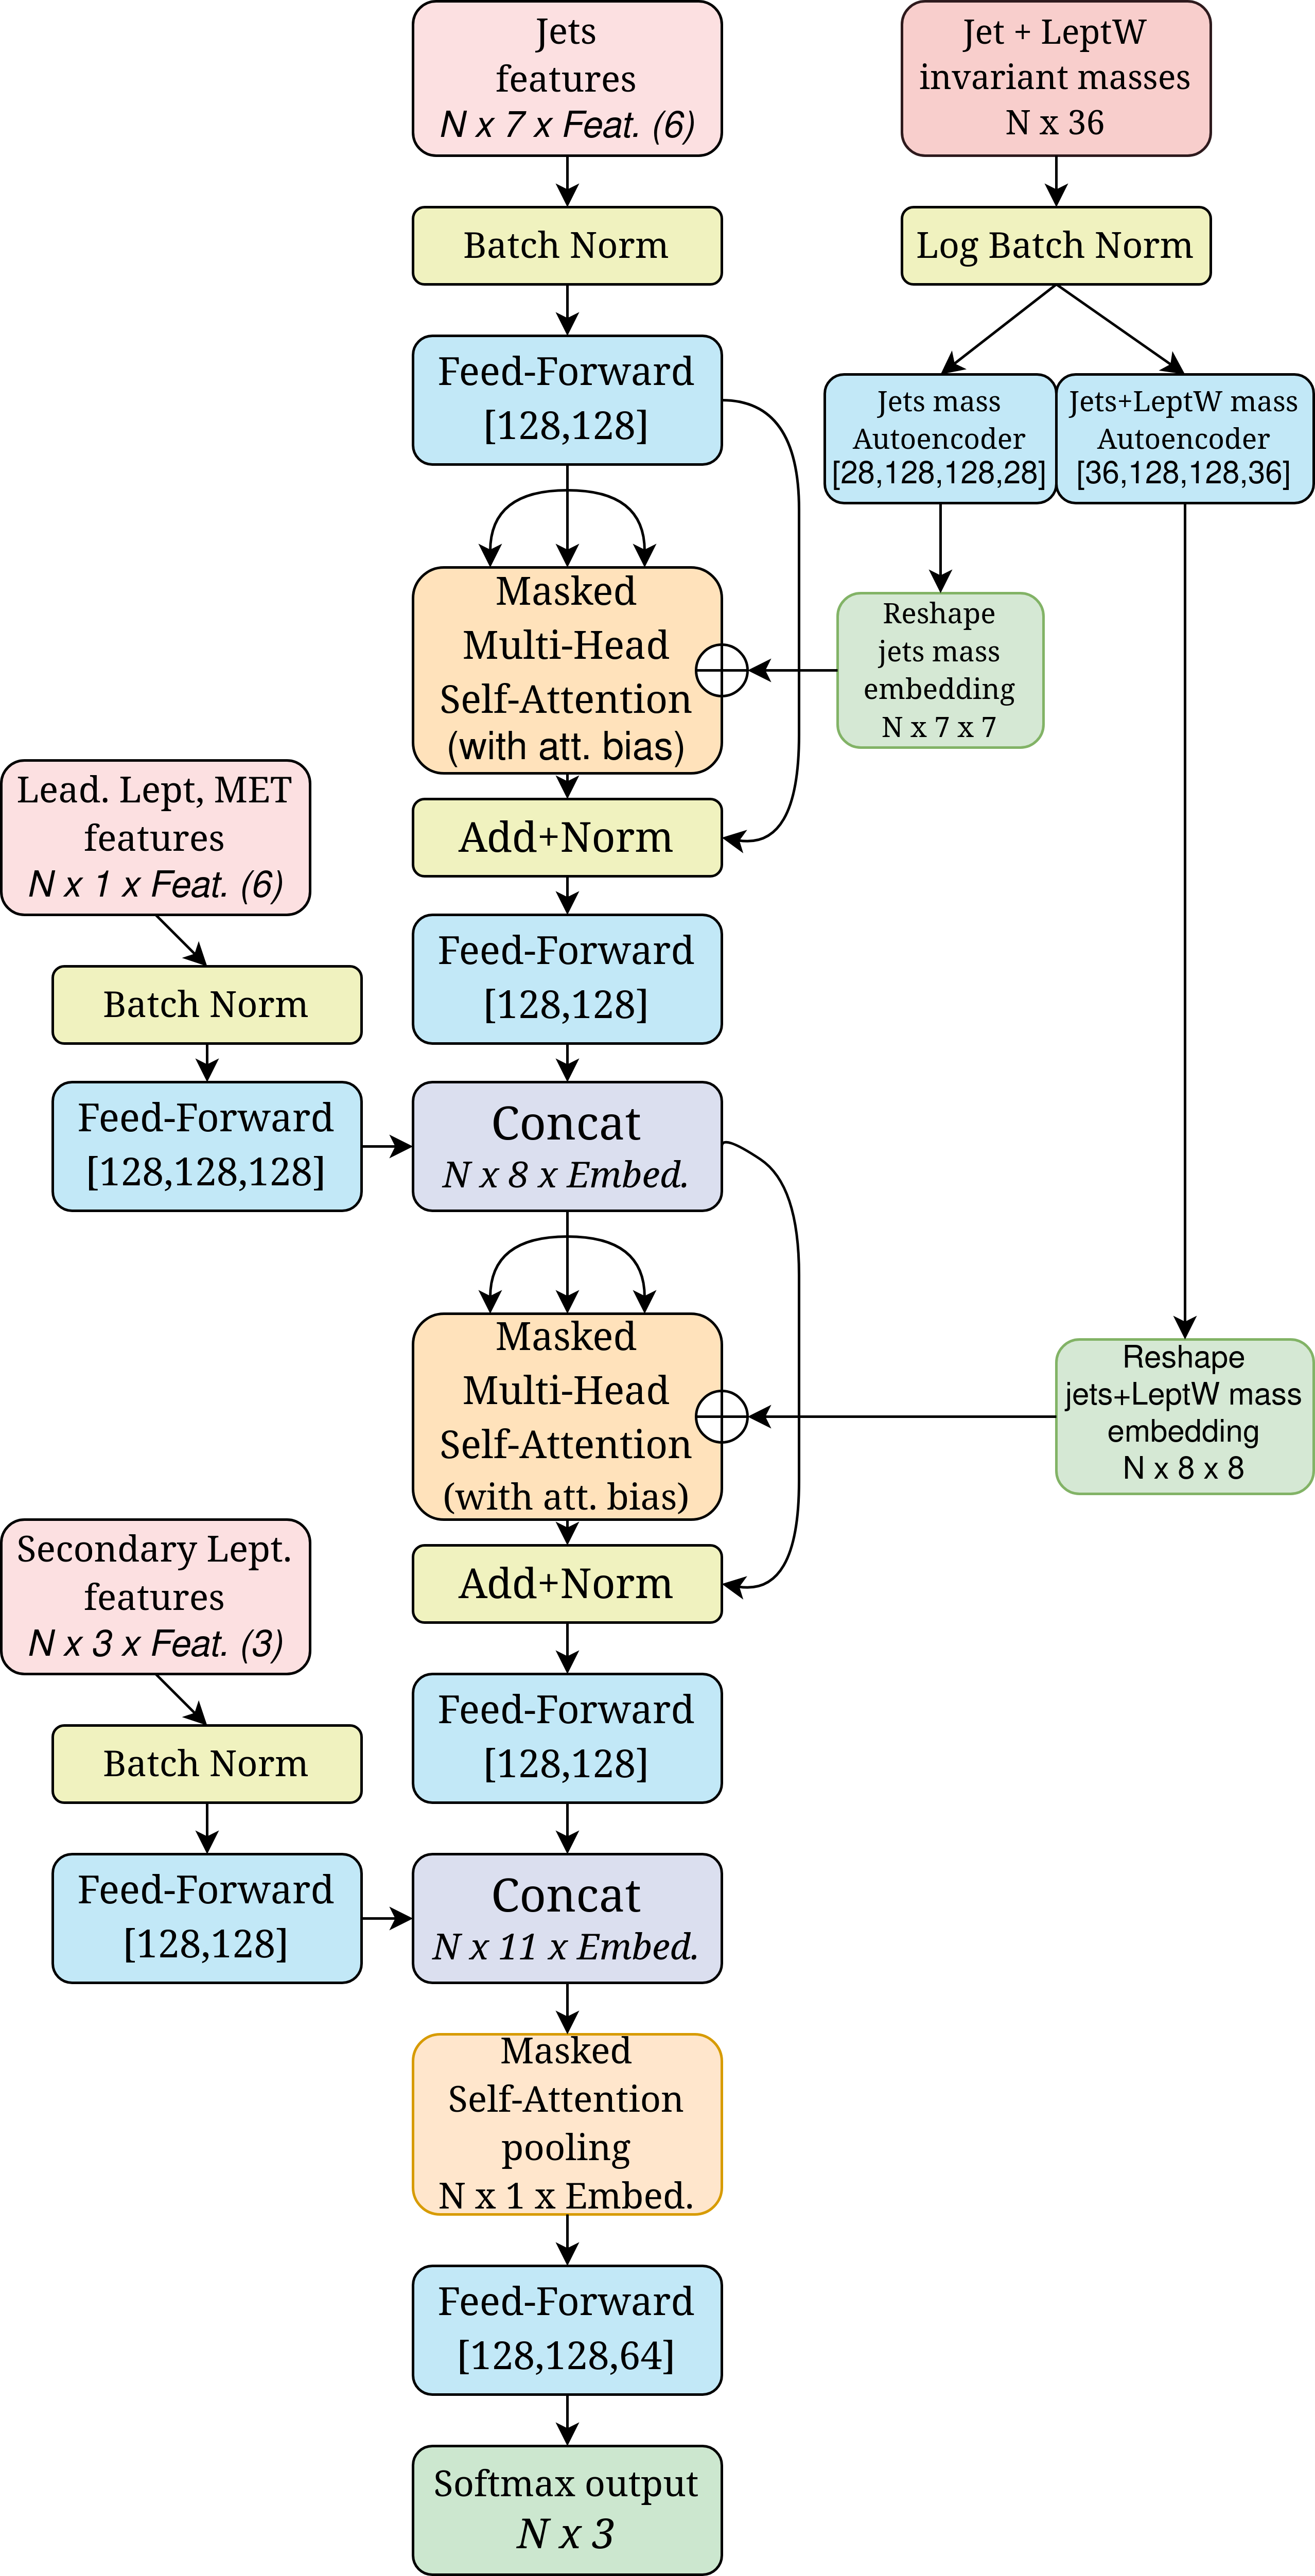
\includegraphics[height=0.805\textheight]{fig//chap09-sigback/SBANet.png}
    %\caption{SBANet}
    \label{fig:SBANet}
\end{figure}

\begin{minipage}{0.58\linewidth}
\begin{table}[H]
    \centering
    \fontsize{11.8pt}{11.8pt}\selectfont
    \begin{tabular}{l|l}
    \toprule
        \textbf{Head} & \textbf{Input features} \\
    \midrule
         Jets & $[p_T,\eta,\phi,\text{bTag},\text{CvB},\text{CvL}]$ \\
         \midrule
         LeptW & $[p_T^\ell,\eta^\ell,\phi^\ell,p_T^\nu,\eta^\nu,\phi^\nu]$\\
         \midrule
         Sec. Lept.& $[p_T,\eta,\phi]$ \\
         \midrule
         Masses & 36 Jets+LeptW inv. masses\\
         \bottomrule
    \end{tabular}
    %\caption{Caption}
    \label{tab:sbanet_inputs}
\end{table}
\end{minipage}
\hfill
\begin{minipage}{0.4\linewidth}
    \begin{table}[H]
    \centering
    \begin{tabular}{l|l}
    \toprule
        Act. function & Swish\\
        Loss& Cross-Entropy\\
        Optimizer & RAdam \\
        Learn. rate & 0.001\\
        Batch size & 20000\\
        Dropout  & 0.02\\  
        \bottomrule
    \end{tabular}
\end{table}
\end{minipage}
\captionof{figure}{SBANet schematics, inputs, and hyper-parameters.}

\begin{figure}[H]
    \centering
    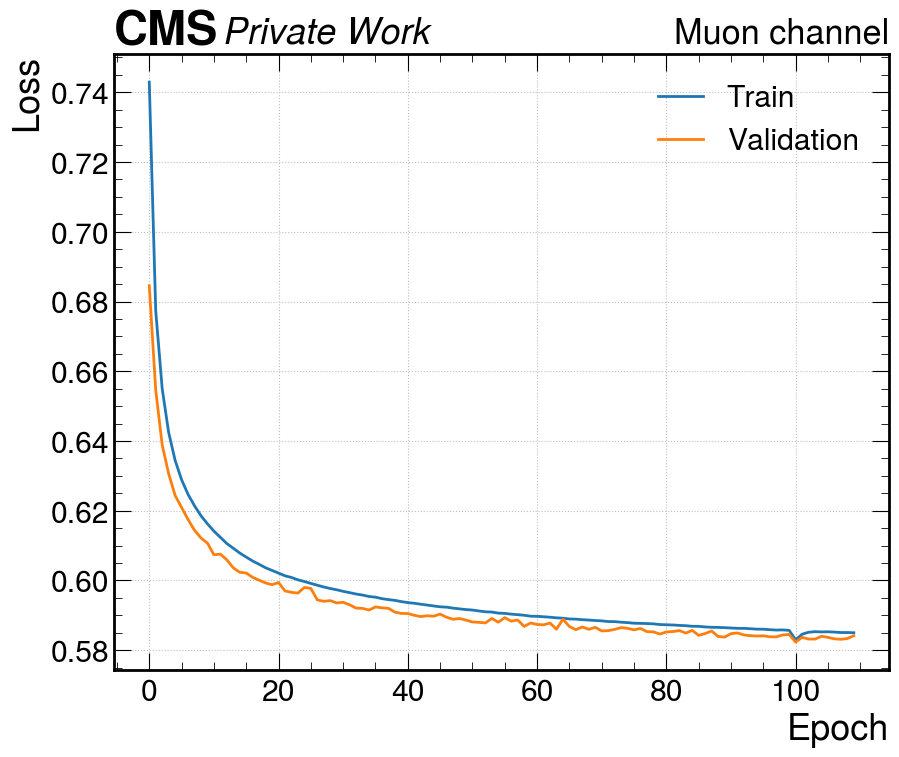
\includegraphics[height=0.48\textheight]{fig//chap09-sigback/loss_Muon.png}
    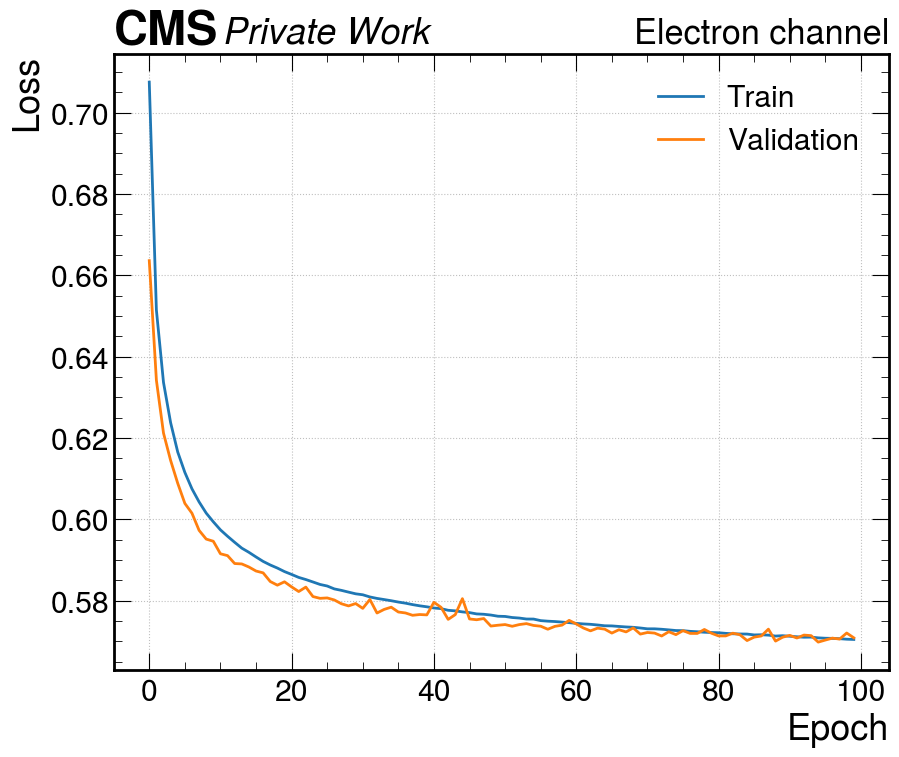
\includegraphics[height=0.48\textheight]{fig//chap09-sigback/loss_Electron.png}
    \caption{SBANet training and validation loss for the muon and electron channel.}
    \label{fig:SBANET_loss}
\end{figure}


\begin{figure}[H]
    \centering
    \includegraphics[height=0.48\textheight]{fig//chap09-sigback/stack_score_muons.png}
    \includegraphics[height=0.48\textheight]{fig//chap09-sigback/stack_score_electrons.png}
    \caption{Stacked distribution of the SBANet scores for each process and signal sensitivity ($\bm{Q}$) plot in the muon (top) and electron (bottom) channel.}
    \label{fig:SBANET_scores}
\end{figure}

\section{Signal rate extraction}
To extract the $\PW \to cb$ rate, the SBANet score is employed to perform a template fit.

\begin{minipage}{\linewidth}
\begin{minipage}{0.43\linewidth}
\begin{table}[H]
    \centering
    \begin{tabular}{l|cc}
    \toprule
        \textbf{Channel} & $\bm{Q}$ & $\dfrac{\bm{\sigma[R(W \to cb)]}}{\bm{R(W \to cb)}}$ \\
        \midrule
         Muon & 98.50 & 10.1\%\\
         Electron & 68.65 &  11.3\%\\
         Combined & 177.15 & 7.5\%\\
         \bottomrule
    \end{tabular}
    \caption{signal sensitivity and estimate of the statistical uncertainties on the $\PW \to cb$ rate of each channel.}
    \label{tab:stat_unc}
\end{table}
    
\end{minipage}
\hfill
\begin{minipage}{0.52\linewidth}
    To expand the region with the highest signal purity, the scores are transformed with the inverse hyperbolic tangent function and then binned in such a way as to maximize the signal sensitivity, maintaining at least one event in each bin.
    Even before executing the fit, the statistical uncertainties on the $\PW \to cb$ rate can be estimated through the signal sensitivity.
\end{minipage}

    
\end{minipage}




\iffalse
\begin{equation*}
    \begin{aligned}
        Q&=98.5 &\implies \frac{\sigma[R(\PW \to cb)]}{R(\PW \to cb)}&\sim 10.1\% & (\text{Muon channel})\\
        Q&=44.1 &\implies \frac{\sigma[R(\PW \to cb)]}{R(\PW \to cb)}&\sim 15.0\% & (\text{Electron channel})\\
        Q&=142.6 &\implies \frac{\sigma[R(\PW \to cb)]}{R(\PW \to cb)}&\sim 8.4\% & (\text{Combined})\\
    \end{aligned}
\end{equation*}
\fi

\paragraph*{Template fit}
The statistical uncertainties on the $\PW \to cb$ rate are derived using the profile likelihood method using the Asimov dataset, as described in Sec. \ref{sec:profile} .

\begin{minipage}{\linewidth}
    \begin{minipage}{0.74\linewidth}
        \begin{figure}[H]
        \centering
        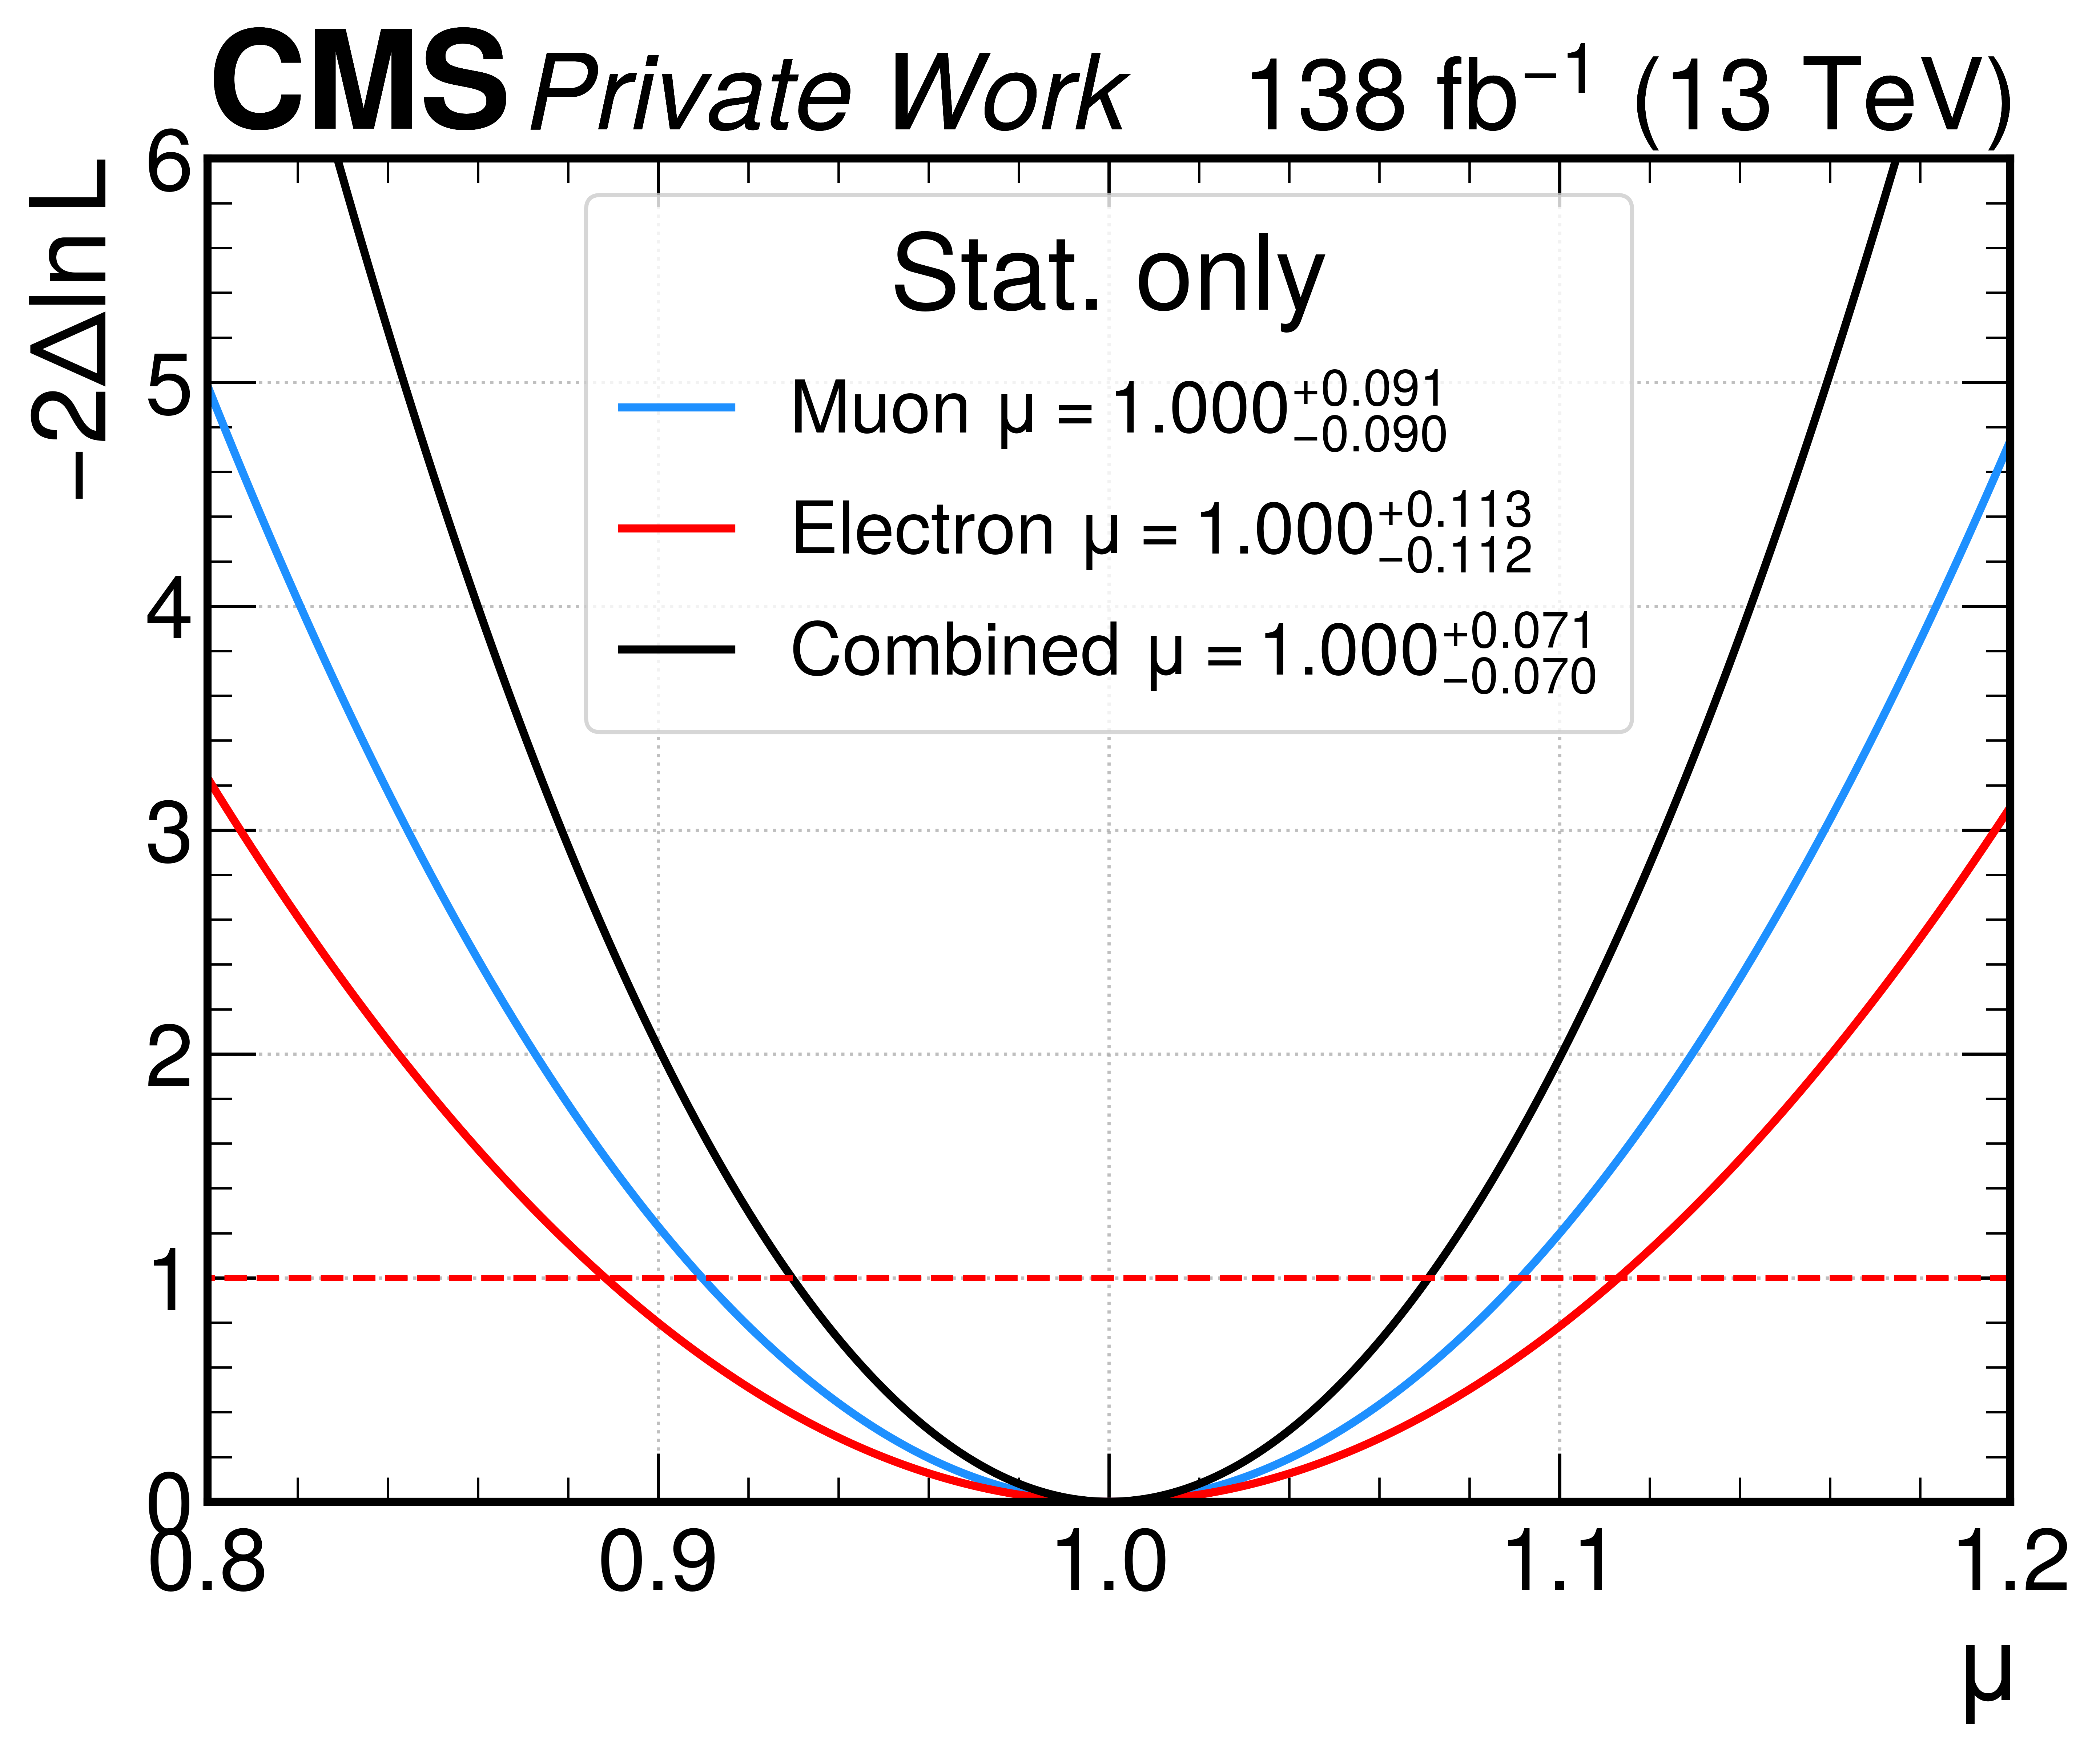
\includegraphics[width=\linewidth]{fig//chap09-sigback/stat_like.png}
        
        \label{fig:enter-label}
        \end{figure}
    \end{minipage}
    \hfill
    \begin{minipage}{0.25\linewidth}
        
        \begin{table}[H]
            \centering
            \begin{tabular}{l|c}
                \toprule
                \multicolumn{2}{c}{\textbf{Rate Stat. Unc.}} \\
                \midrule
                 Muon & 9.0\% \\
                 Electron & 11.2\% \\
                 Combined & 7.0\% \\
                 \bottomrule
            \end{tabular}
            \label{tab:my_label}
        \end{table}
    \end{minipage}
    \captionof{figure}{Profile likelihood on the SBANet score templates in the muon channel, electron channel, and combined.}
\end{minipage}


\subsection{Systematic uncertainties}

In this analysis, the most relevant systematic uncertainties are the following:

\begin{itemize}
    \item \textbf{b/c-tagging uncertanties} 
    The derivation of the b-tagging scale factors, described in Sec. \ref{par:tag_corr}, is subject to systematical uncertainties. The primary sources are the following:
    \begin{itemize}
        \item[\ding{111}] \textit{Sample purity}: The purity of the samples used to compute the light flavor SFs can be compromised by the contamination of heavy flavor jets associated with the Z boson, while for the heavy flavor SFs, the contamination of light jets in the $\ttbar$ sample can occur due to the production of additional partons.\\
        To take into account the uncertainties on the contamination, the rate of $\ttbar$ events produced in association with two or more additional partons and the fraction of heavy flavor jets in the Z+Jets samples are varied of $\pm 20\%$
        
        \item[\ding{111}] \textit{Statistical uncertainties} This source accounts for the statistical fluctuations in different SFs bins that affect the more low-populated regions like the ones with high values of b-tag score

        

        \iffalse
        \item[\ding{111}] \textit{Theoretical MC uncertainties} Uncertainties related to the parameter of the generator like the renormalization scale and the parton shower settings
        \fi
    \end{itemize}
    \item \textbf{JES/JER} Uncertainties related to the jet energy scale and resolution corrections described in Sec. \ref{par:JERC}.

    \item \textbf{Luminosity} Uncertainties on the RunII luminosity: 1.6\%
    \item \textbf{Channel acceptance} Uncertainties on the acceptance of each signal region: 1\%(2\%) Muon(Electron) channel.
    \item \textbf{$\ttbar$ cross-section} Uncertainties on the $\ttbar$ cross-section: 5\%
\end{itemize}
The impact of the systematic uncertainties is evaluated using the profile likelihood method with normal priors for each nuisance.
\begin{table}[H]
    \centering
    \begin{tabular}{l|c}
    \toprule
    \textbf{Uncertainties} & \textbf{Impact}\\
    \midrule
         Statistical   & 7\% \\
         \midrule
         b-tagging   & 7\% \\
         c-tagging   & 4\% \\
         JES/R   & 3\% \\
         Lumi+XSec+Acceptances  & 2\% \\
         \midrule
         Total   & 11\%\\
         \bottomrule
    \end{tabular}
    \caption{Impact of the systematic uncertainties and total uncertainties on the $\PW \to cb$ rate determination.}
    \label{tab:res}
\end{table}

